\documentclass{standalone}

\usepackage{tikz}
\usetikzlibrary{decorations.markings}
\begin{document}



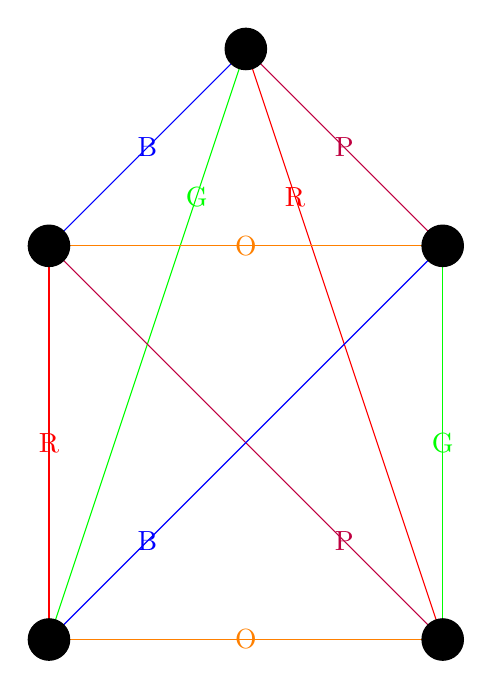
\begin{tikzpicture}[scale=2.5]



\draw[blue] (3,5)-- node {B} (2,4);
\draw[green] (3,5)-- node [near start] {G} (2,2);
\draw[red] (3,5) -- node [near start] {R} (4,2);
\draw[purple] (3,5)-- node {P} (4,4);

\draw[red] (2,4)-- node {R} (2,2);
\draw[orange] (2,4)-- node {O} (4,4);
\draw[purple] (2,4)-- node[near end] {P} (4,2);

\draw[blue] (2,2)-- node[near start] {B} (4,4);
\draw[orange] (2,2)-- node {O} (4,2);
\draw[green] (4,2)-- node {G} (4,4);


\filldraw (2,2) circle(3pt);
\filldraw (2,4) circle(3pt);
\filldraw (4,2) circle(3pt);
\filldraw (4,4) circle(3pt);
\filldraw (3,5) circle(3pt);



\end{tikzpicture}
\end{document}
